\subsubsection{Fibonacci Line Search}The Fibonacci line search and the golden section search are both based on a fundamental method of interval selection. As opposed to the dichotomous line search, these methods only require one function evaluation per iteration. This is achieved by reusing one of the function evaluations performed in the previous iteration.

An example of this interval system is shown in \figref{fibonacciIntervalSystem} where the first iteration, marked in green, assuming some bracket, \si{[x_{L},\ x_{U}]}, produces two intervals with equal lengths of \si{I_1}. Either the right or the left interval is then chosen as the new bracket. In \figref{fibonacciIntervalSystem} \si{f(x_a) > f(x_b)}, therefore the right interval must contain the minimizer, so long as there is only one minimum within the bracket. Thus, the new bracket is set: \si{[x_{L},\ x_{U}] = \si{[x_{a},\ x_{U}]}}.\\
In the case that \si{f(x_a) = f(x_b)}, either \si{x_a} or \si{x_b} can be set as the new boundary.

Within this bracket one function evaluation has already taken place (the circled red dot), this interval can be reused and only one further evaluation of \si{f(x)} is needed to proceed with the next iteration.

\begin{figure}[H] 
	\centering
	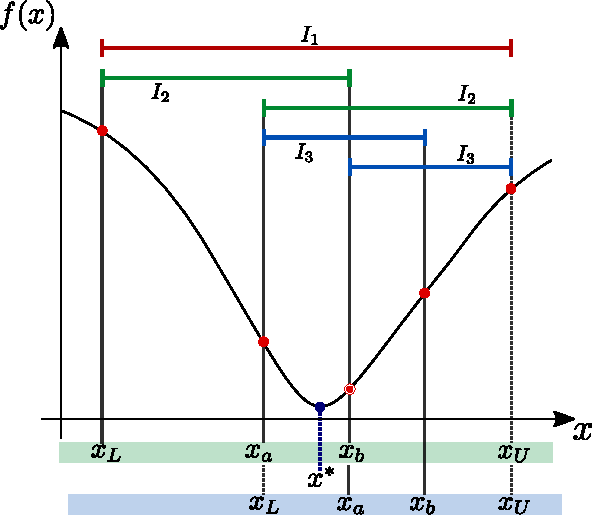
\includegraphics[width=.5\textwidth]{figures/fibonacciIntervalSystem}
	\caption{The function, \si{f(x)}, is only evaluated at the points indicated by red dots and the function f(x) is obviously unknown in the process. First iteration is marked in green and the second in blue. \si{x^*} denotes the local minimizer and \si{I} is used to relate length of the intervals, showing that the two intervals in each iteration are equal.}
	\label{fibonacciIntervalSystem}
\end{figure}

If this procedure is repeated with numerous iterations, a series of interval lengths is produced. From \figref{fibonacciIntervalSystem} the relation between successive interval lengths can be described as \si{I_1 = I_2 + I_3}, or in general for any iteration, \si{k}, as \si{I_k = I_{k+1} + I_{k+2}}.\\
With this as a basis, different ratios between \si{I_{k+1}} and \si{I_{k+2}} can be chosen, such as the golden section or the Fibonacci numbers.\\
If for the last n-th iteration, \si{I_{n+2}} is assumed to be zero, then \si{ I_n  = I_{n+1} + I_{n+2}  = I_{n+1} } and the following sequence of intervals emerges.
%
\begin{flalign}
  \si{I_{n+1}}              &=  \phantom{\si{\ I_{n+1}  + I_{n+2}            =}}  \si{ 1 I_n  = F_0 I_n } &\nonumber\\
  \si{I_{n}}\phantom{_{+1}} &=  \si{ I_{n+1}  + I_{n+2} }                    =  \si{ 1 I_n  = F_1 I_n }   &\nonumber\\
  \si{I_{n-1}}              &=  \si{ I_{n} }\phantom{_{+1}} + \si{ I_{n+1} } =  \si{ 2 I_n  = F_2 I_n }   &\nonumber\\
  \si{I_{n-2}}              &=  \si{ I_{n-1}  + I_{n} }\phantom{_{-1}}       =  \si{ 3 I_n  = F_3 I_n }   &\nonumber\\
  \si{I_{n-3}}              &=  \si{ I_{n-2}  + I_{n-1} }                    =  \si{ 5 I_n  = F_4 I_n }   &\nonumber\\
  \si{I_{n-4}}              &=  \si{ I_{n-3}  + I_{n-2} }                    =  \si{ 8 I_n  = F_5 I_n }   &\nonumber\\
  \phantom{I_{n-4}}         &\phantom{..}\vdots                                                           &\nonumber\\
  \si{I_{k}}                &=  \si{ I_{k+1} + I_{k+2} = F_{n-k+1} I_n }                                  &\nonumber\\
  \phantom{I_{n-4}}         &\phantom{..}\vdots                                                           &\nonumber\\
  \si{I_{1}}                &=  \si{ I_{2} + I_{3} = F_n I_n }                                            &
  \label{fibonacciNumbers}
\end{flalign}
%
Where:\\
\begin{tabular}{ l l l l}
& \si{F_n}                               & is the largest Fibonacci number used.     &\\
& \si{\{ \ F_0,\ F_1,\ \dots\ F_n \ \}}  & is the Fibonacci sequence up to \si{F_n}  &%, \si{\{\ 1,\ 1,\ 2,\ 3,\ 5,\ \dots\ F_n  \}}  
\end{tabular}

For the last expression in \eqref{fibonacciNumnbers}, the size of the first bracket, \si{I_1}, is known and the last interval, \si{I_n}, can be chosen as the precision of the search. From this, the largest Fibonacci number needed can be found as \si{F_n = \frac{I_1}{I_n}}, and the remaining intervals can be calculated progressively during each iteration by use of the appropriate numbers in the Fibonacci sequence.\\
In \figref{fibonacciLineSearchComprehensive} an example implementation is shown where each iteration contains \si{x_a} and \si{x_b}. In the iterations where \si{x_a} is chosen as the new \si{x_{L}} it is marked with a red circle and for \si{x_b} chosen as new \si{x_{U}} a blue circle is used. It shows clearly shows how each iteration only requires one function evaluation.

\begin{figure}[H] 
	\centering
	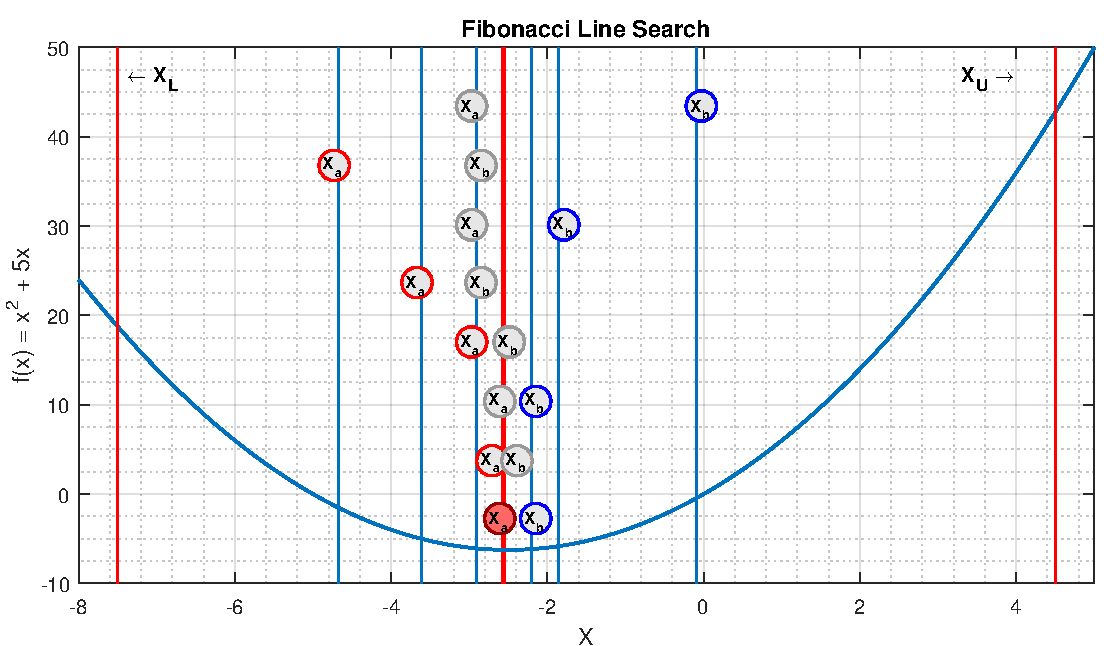
\includegraphics[width=.8\textwidth]{figures/fibonacciLineSearchComprehension}
	\caption{Fibonacci line search where the first iteration is at the top of the graph and each subsequent iteration is listed one line at a time downward. New \si{x_{L}} is marked with a red circle and new \si{x_{U}} with a blue circle. The chosen minimizer is marked in red at the bottom.}
	\label{fibonacciLineSearchComprehensive}
\end{figure}

To see the benefits of using the Fibonacci line search rather than the more rudimentary dichotomous line search, the one-dimentional implementations are compared between \figref{fibonacciLineSearchPerformance} and \figref{dichotomousLineSearchPerformance}. The precision intervals determining how close each method is to reaching the true minimum are set to approximately the same value. This is done such that the number of function evaluations used for similar results can be compared in the two methods.

\begin{figure}[H] 
	\centering
	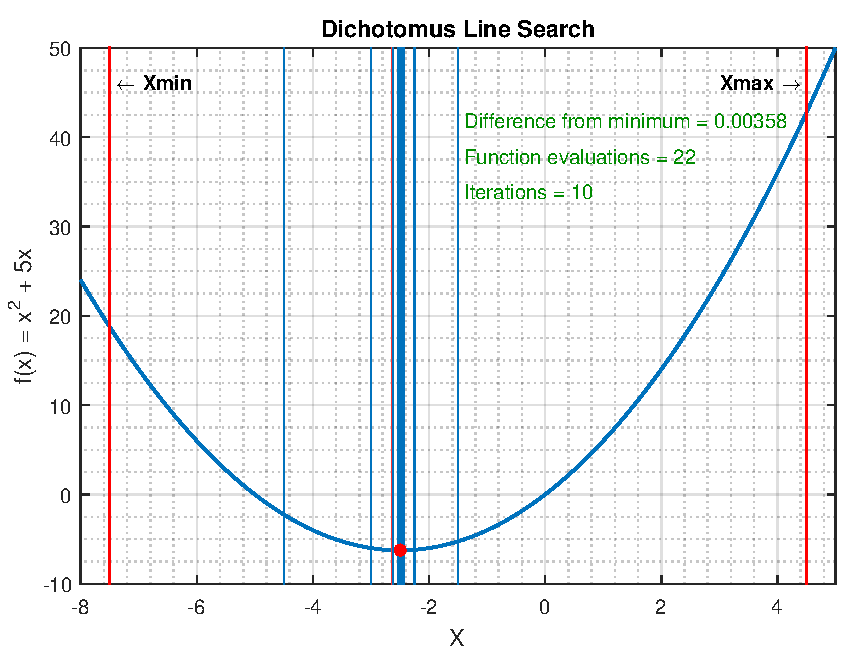
\includegraphics[width=.65\textwidth]{figures/dichotomousLineSearchPerformance}
	\caption{Example showing iterations and function evaluations used to obtain a given performance of the dichotomous Line Search.}
	\label{dichotomousLineSearchPerformance}
\end{figure}

In the dichotomous line search fewer iterations are used because each iteration almost cuts the bracket in half for each iteration. However, since each iteration requires two evaluations of \si{f(x)}, the final number of function evaluations exceeds that of the Fibonacci line search. This is of course not always true - the location of the minimum in the bracket plays a role. If the minimum lies close to the middle of the bracket the dichotomous line search might get there faster than the Fibonacci line search. However for a broad spectrum of problems the performance of the Fibonacci line search will likely beat that of the dichotomous line search.

\begin{figure}[H] 
	\centering
	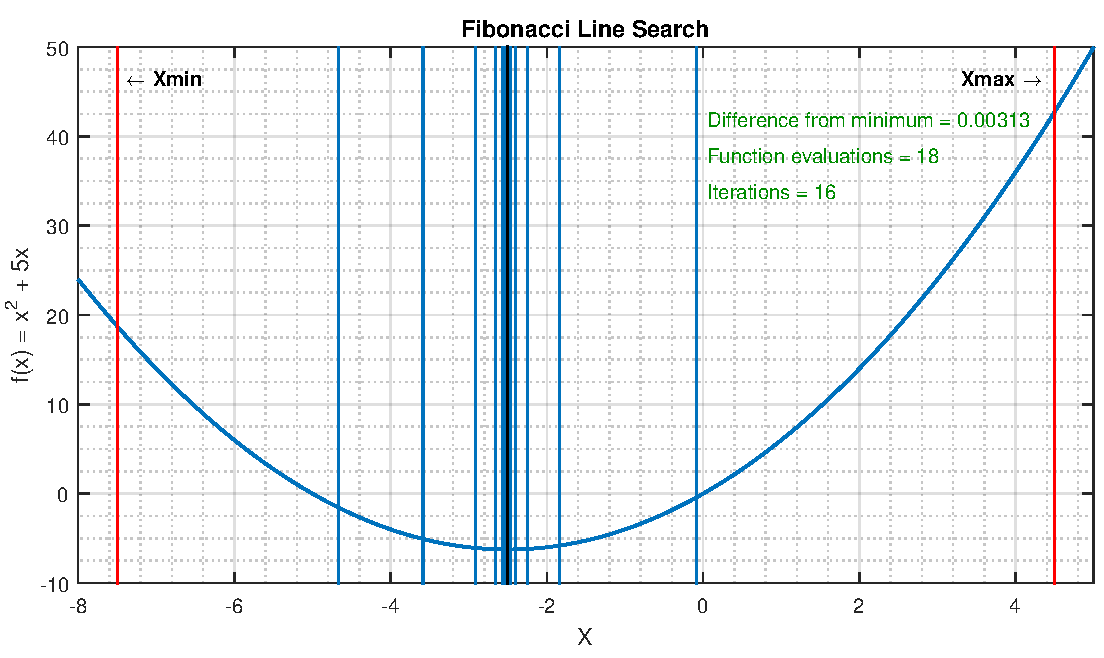
\includegraphics[width=.65\textwidth]{figures/fibonacciLineSearchPerformance}
	\caption{Example showing iterations and function evaluations used to obtain a given performance of the Fibonacci Line Search.}
	\label{fibonacciLineSearchPerformance}
\end{figure}

The lower number of function evaluations makes the Fibonacci line search superior in this case. In these examples the function can be analytically evaluated and the minimization problem can be solved analytically in one iteration. This is however not the case for a cost function representing mean squared error between simulation and reality for each change in one or more parameters. Such a cost function requires a simulation for each and every function evaluation. This is a time-expensive task which is why Fibonacci line search is chosen for the task at hand.